\chapter{Chemodynamical Analysis of Six Low-Metallicity Stars in the Galactic Halo}\label{chap:introduction}




\section{Results and Discussion}\label{sec:discussions}
  
\subsection{Chemical Abundance Comparison with Literature Data}
 

To identify any possible chemical peculiarities in our sample, we compared our
determinations with data from the literature. Figure \ref{fig:abund} shows some
of the light-element abundances, compared to C-normal stars taken from
\citet{2013ApJ...762...26Y}. The detectable light-elements have similar
abundance ratios to those reported in literature halo stars, suggesting that our
sample stars have been likely formed from a well-mixed gas cloud.

All our sample stars have been evolved into the red giant branch, suggesting that some internal mixing occurred and thus the
atmospheric carbon abundances have been altered.  \citet{2014ApJ...797...21P}
studied a sample of 505 metal-poor stars and developed a correction procedure that
recovers the initial atmospheric carbon abundance.  We obtained high $[C/Fe]_{corr}$ values
for J1630+0953 and J2216+0246 ($[C/Fe]_{corr}$ = +0.62 and 0.42 dex,
respectively), which brings the final abundances to [C/Fe]=1.26 and
0.70. From these final values and the definition of the CEMP
(CEMP [C/Fe] $\geq 0.7$; \citealt{2007ApJ...655..492A}), we classify J1630+0953 and J2216+0246 as
carbon-enhanced metal-poor stars, while the rest of our program stars are
carbon-intermediate.

\begin{figure}[!ht]
\centering
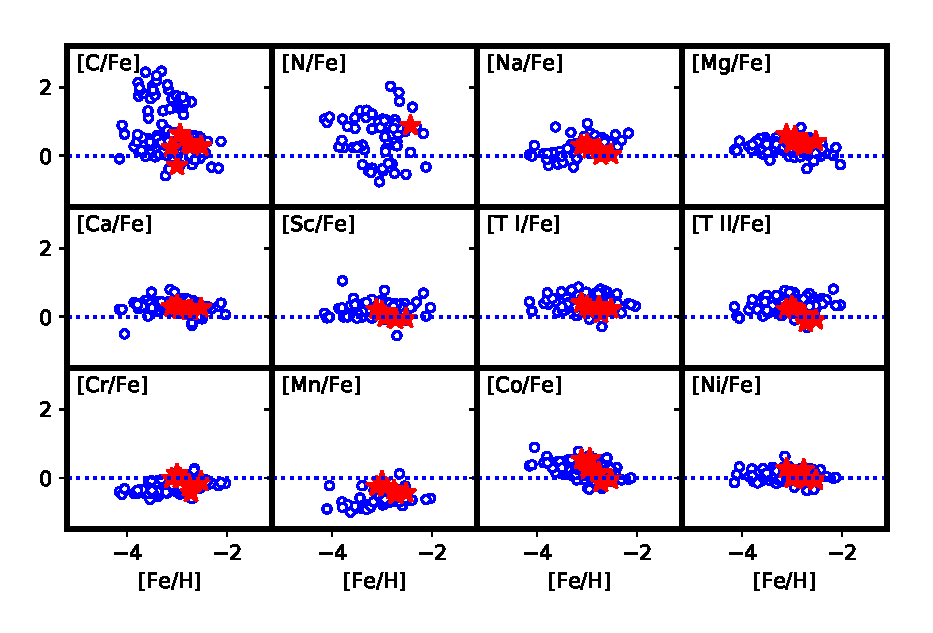
\includegraphics[width=\textwidth, angle=0]{light_elements.eps} 
\caption{Selected light-elements abundances of our sample stars (red filled
stars) overlaid with [X/Fe] of carbon-normal metal-poor stars adopted
from \citet{2013ApJ...762...26Y} (blue open circles). Our derived [X/Fe]
show no significant differences compared to the literature data. [C/Fe]
values do not represent the carbon abundances of the natal gas.}
\label{fig:abund}
\end{figure}



The substantial depletion of carbon in J1630+0953 and J2216+0246 suggests that
the chemical patterns observed in these two stars should be accompanied with
nitrogen enhancement. However, we were only able to detect nitrogen in the
spectrum of J1630+0953 ([N/Fe]=0.88), which is in line with its
evolutionary status, while J2216+0246 spectrum show no reliable CN features.  


\begin{figure}[!ht]
\centering
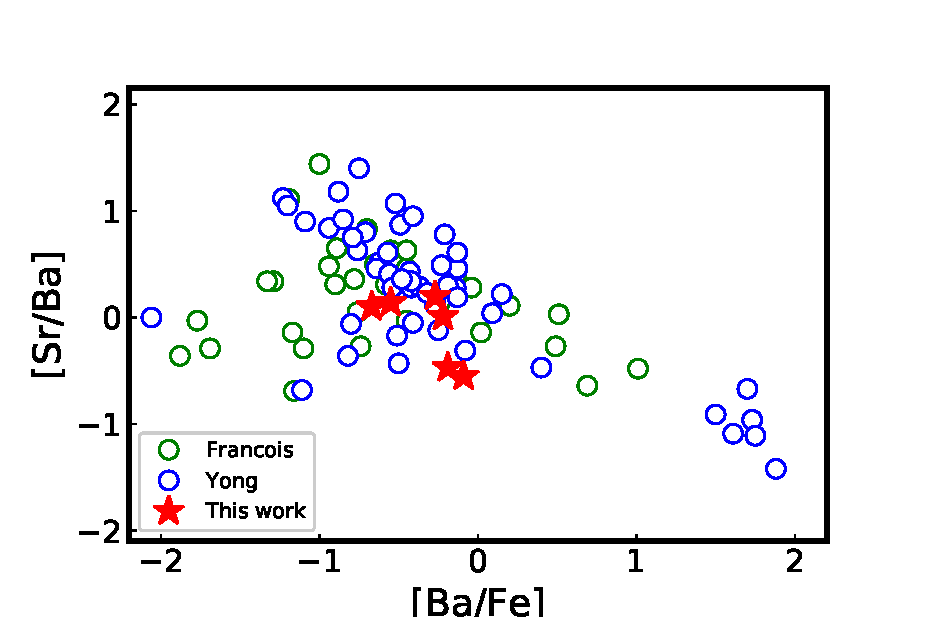
\includegraphics[width=\textwidth, angle=0]{Sr_Ba.eps} 
\caption{The determined abundance ratios [Sr/Ba] of our sample stars (red filled stars), versus [Ba/Fe]. The green and blue open circles denote literature data adapted from \citet{2007A&A...476..935F} and
\citet{2013ApJ...762...26Y}, respectively.}
\label{fig:Sr_Ba}
\end{figure}

We have determined chemical abundances for up to nine neutron-capture elements
in our sample stars. Of particular interest, the observed Sr and Ba abundances
could help us better understand their nucleosynthesis pathway(s), considering
that Sr (first s-process peak) may be synthesized by the main or weak s-process,
while Ba (second s-process peak) primarily synthesized by the main s-process
\citep{2003ApJ...588.1099Q, 2008ApJ...687..272Q, 2011A&A...530A.105A,
2014ApJ...797..123H}. Furthermore, \citet{2009ApJ...696..797C,
2011ApJS..197...17C} and \citet{2012ApJ...747....2L} predicted that low and
high [Sr/Ba] ratios could help discriminate between low-mass and
massive metal-poor AGB stars, respectively. This further suggests that the
production of Sr and Ba are linked to various astrophysical sites. On the
other hand, \citet{2013ApJ...766L..13A} suggested that these elements could
be synthesized in the same event, and the observed [Sr/Ba] ratios can
be explained by the stars collapse time into a black-hole. 

Figure \ref{fig:Sr_Ba} shows the [Sr/Ba] abundance ratios of our program
stars (filled red stars) and carbon-normal stars from
\citet{2007A&A...476..935F} (green open circles) \citet{2013ApJ...762...26Y}
(blue open circles), as a function of [Ba/Fe]. All of the sample stars
show no significant differences from the trends presented by
\citet{2007A&A...476..935F} and \citet{2013ApJ...762...26Y}. However, abundances
from elements in the first s-process peak in J0326+0202 ([Sr/Ba] = 0.14)
and J1413+1727 ([Sr/Ba] = 0.20) appear to be enriched more than the
second peak, thus an additional process is required to explain these high
[Sr/Ba] ratios.  J1630+0953 and J2216+0246 satisfied the CEMP definition
([C/Fe] $\geq 0.7$;\citealt{2007ApJ...655..492A}). In addition,  we
determined low Ba abundances ([Ba/Fe]$<$ 0.0) for these stars.  Therefore, J1630+0953 and J2216+0246 can be classified as
CEMP-no stars \citep{2005ARA&A..43..531B, 2007ApJ...655..492A, 2014ApJ...797...21P}. 


\begin{figure}[!ht]
\centering
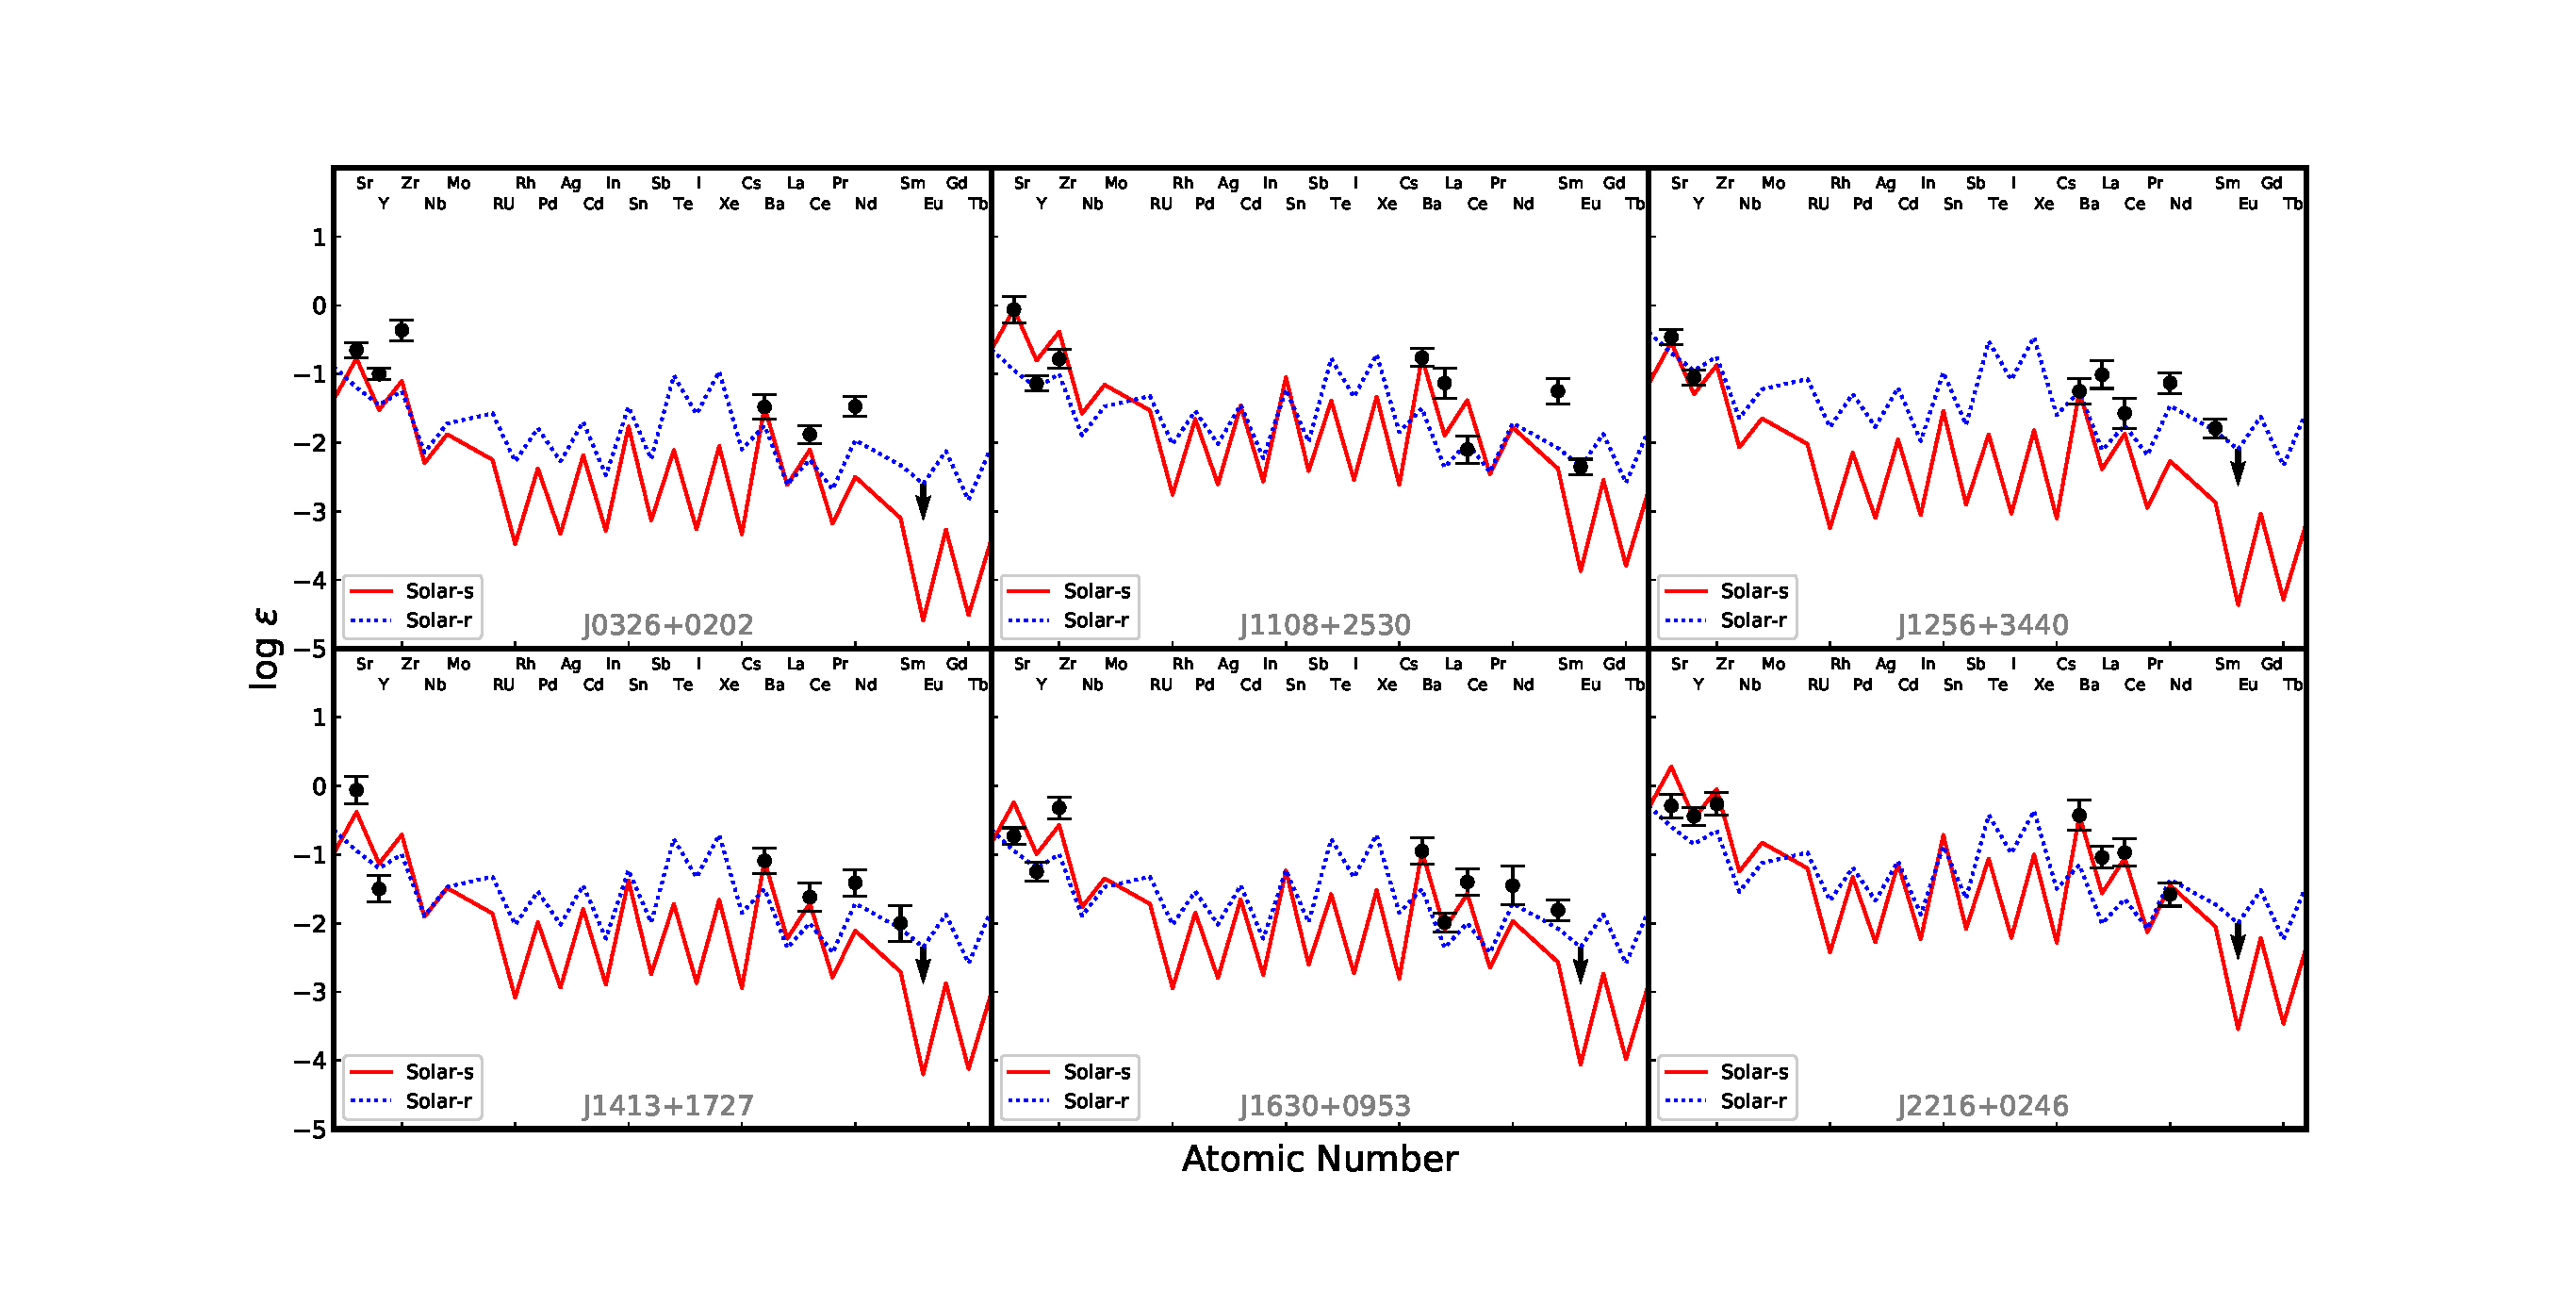
\includegraphics[width=\textwidth, angle=0]{solar_r_s-process.eps} 
\caption{Elemental abundance patterns for the heavy element distribution in our
sample stars (filled circles denote detections, and arrow denotes $3 \sigma$
upper limits derived from \ion{Eu}{2} line), compared with scaled solar system
r- and s-process components adopted from \citet{2000ApJ...544..302B}. The solar
system r-process patterns are scaled to match Eu, and the solar system s-process
patterns are scaled to match Ba.}
\label{fig:solar_r_s-process}
\end{figure}



\begin{figure}[!ht]
\centering
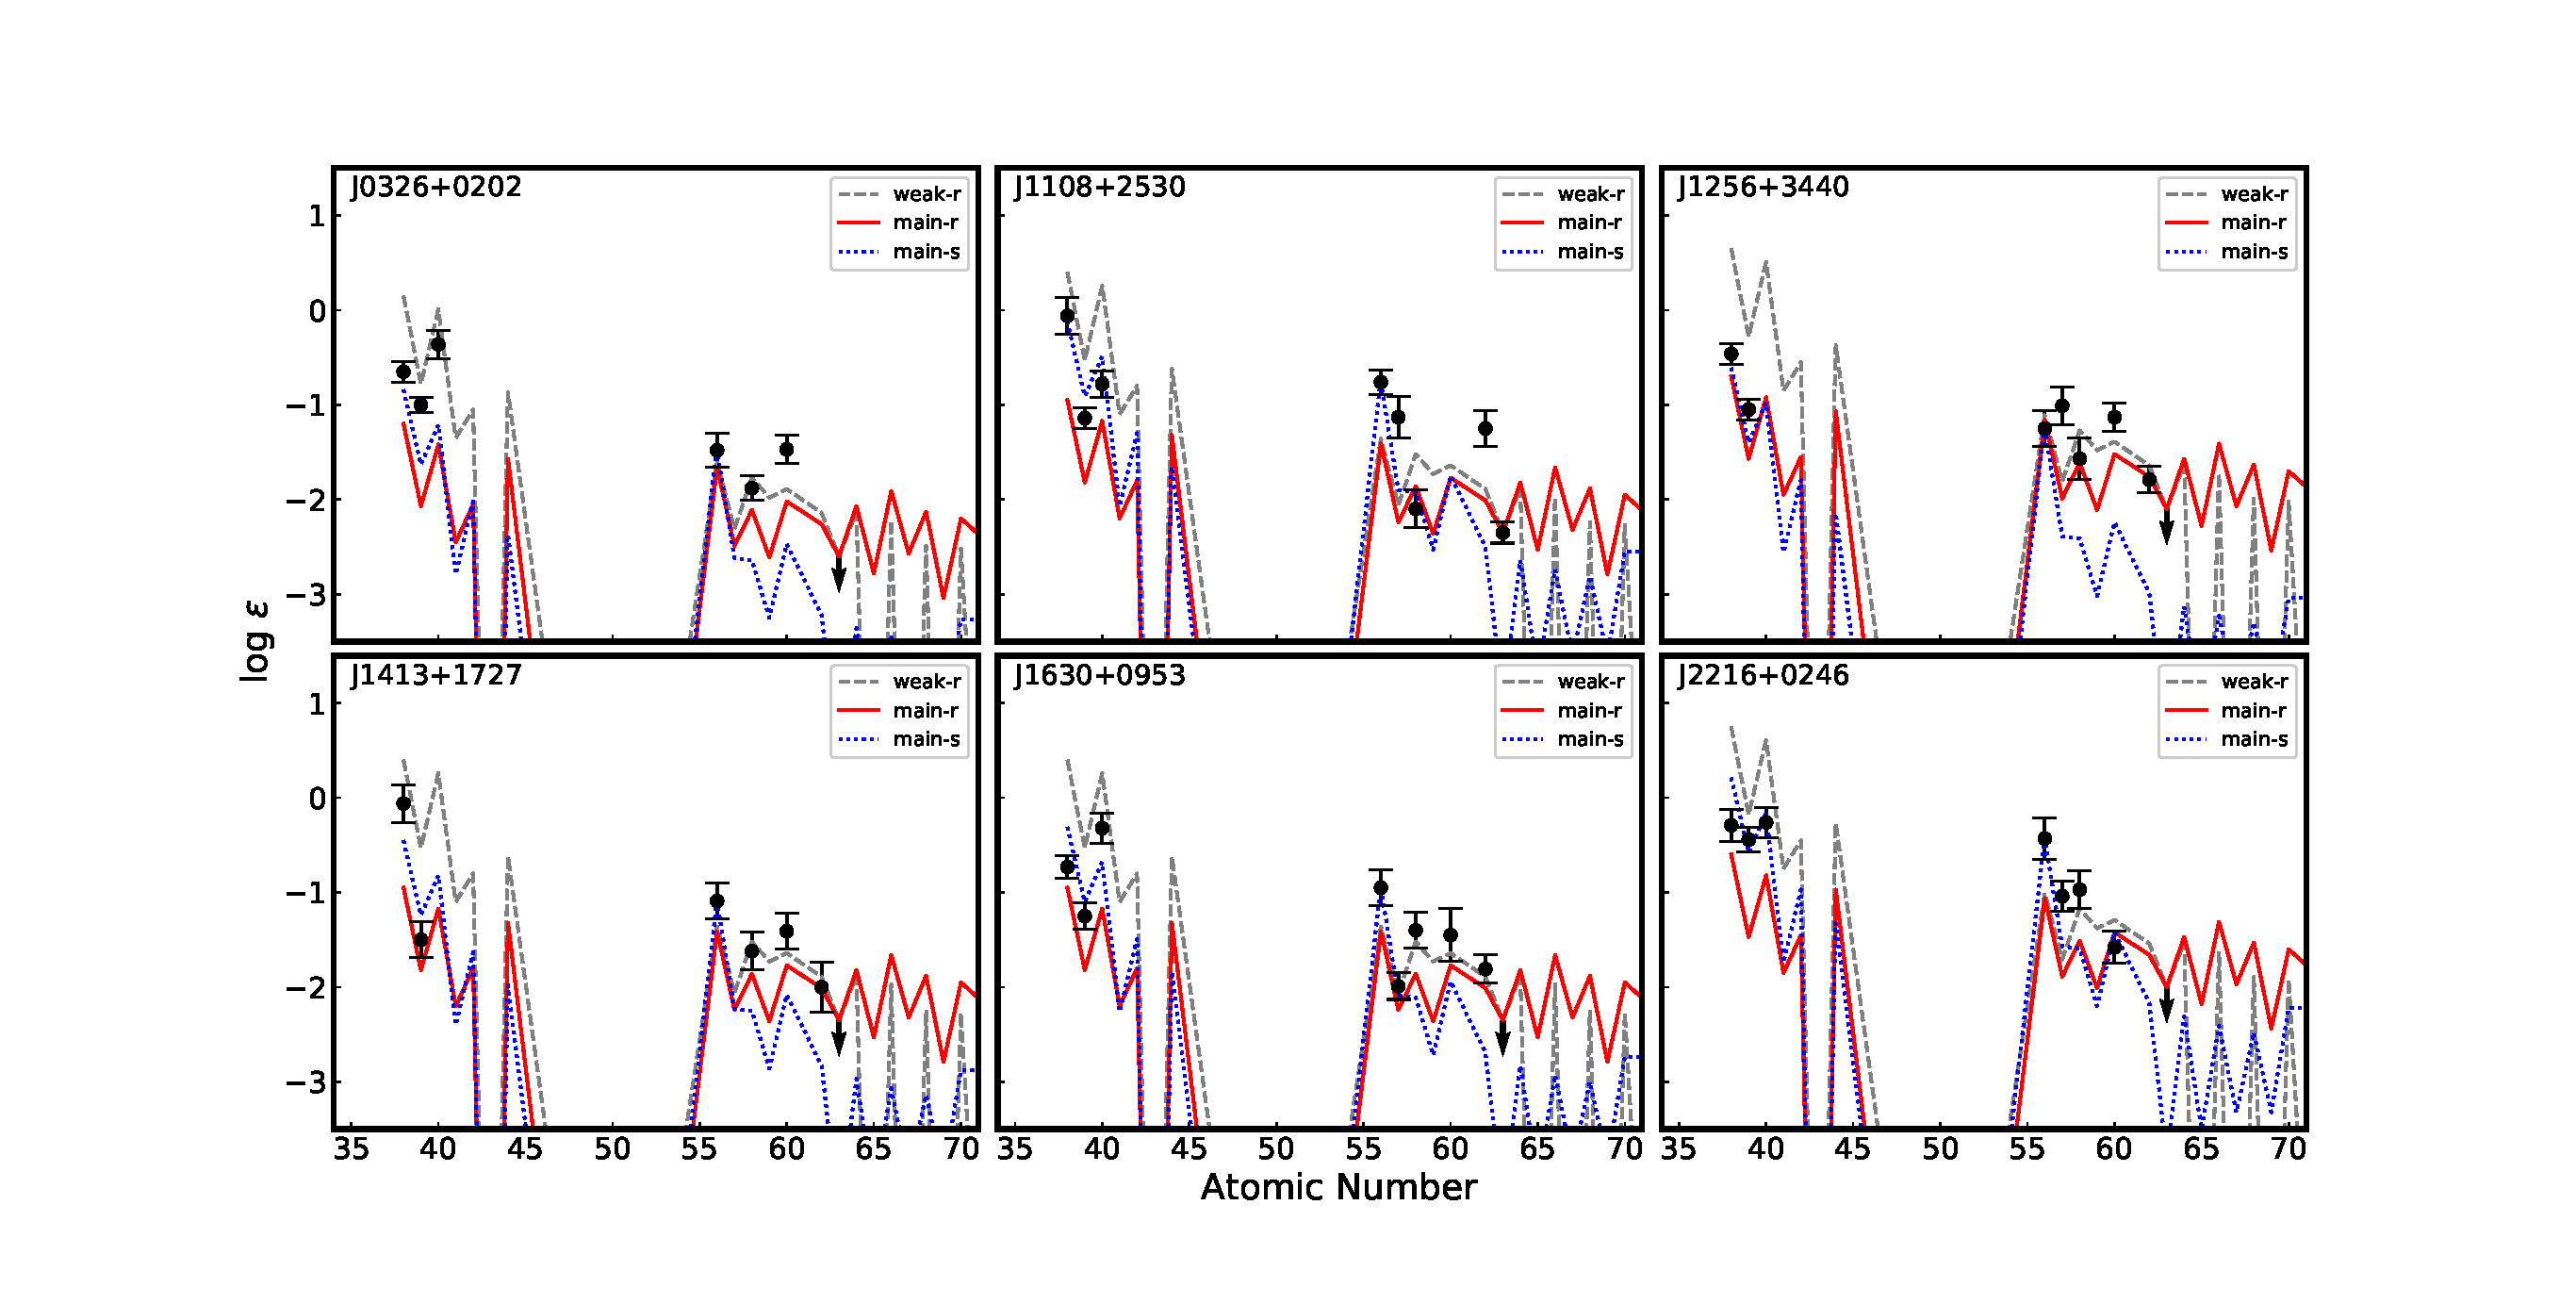
\includegraphics[width=\textwidth, angle=0]{weak_main.eps} 
\caption{Neutron-capture element patterns in our sample stars. Filled circles
denote detections, and arrow denotes $3 \sigma$ upper limits derived from
\ion{Eu}{2} line. The dashed gray line denotes the observed abundances for the
neutron-capture elements in HD122563 \citep{2006ApJ...643.1180H,
2012ApJS..203...27R}. The solid red line denotes the observed abundances for the
neutron-capture elements in CS 22892–052 \citep{2003ApJ...591..936S,
2009ApJS..182...80S, 2009ApJ...698.1963R}. The dotted blue line denotes
predicted yields from s-process nucleosynthesis in TP-AGB stars
\citep{2008ARA&A..46..241S, 2011MNRAS.418..284B}. The physical meaning of these
three lines are discussed in the text.}
\label{fig:weak_main}
\end{figure}

By comparing the observed neutron-capture abundance patterns in our sample
stars with the solar system (SS) r- and s-fractions, we can gain insights into
the nature of their heavy element enrichment. Figure \ref{fig:solar_r_s-process} shows the
heavy element abundance patterns of our sample stars compared with the SS r- and
s-fractions, adopted from \citet{2000ApJ...544..302B}. The SS s-process
components are normalized to match the observed Ba (solid line), and the SS
r-process patterns are normalized to match the observed Eu (dotted line). The
derived abundances for Sr, Y, and Zr (within observational errors) in J0326+0202
seem to be inconsistent with the SS distributions. These discrepancies require
an additional process(es) to interpret the overall neutron-capture abundance
pattern observed in this star. However, these elements seem to be consistent
with the SS s-process distributions for the rest of our sample stars. Heavier
elements (Z $\geqslant 56$) in J0326+0202, J1256+3440,  J1413+1727, and
J1630+0953 are in better agreement with the normalized SS r-process than the
normalized SS s-process. The heavier elements in J2216+0246 seem to favor the
normalized SS s-process. The abundance pattern in J1108+2530 is not in agreement
with the SS abundance pattern.

Figure \ref{fig:weak_main} shows the heavy element abundance patterns in our
sample stars compared with abundance patterns of HD 122563 \citep[the dashed
gray line,][]{2006ApJ...643.1180H, 2012ApJS..203...27R}, CS 22892–052 \citep[the
solid red line,][]{2003ApJ...591..936S, 2009ApJS..182...80S,
2009ApJ...698.1963R}, and predicted yields from s-process nucleosynthesis in
TP-AGB stars \citep[the dotted blue line,][]{2008ARA&A..46..241S,
2011MNRAS.418..284B}. These patterns can be used as weak component of
the r-process (HD 122563), main component of the r-process (CS 22892–052), and
main component of the s-process (TP-AGB yields) representatives
\citep{2014ApJ...784..158R}. The abundance pattern of HD122563 and CS 22892–052
are renormalized to match the observed Eu, and the dotted blue line is
renormalized to match the observed Ba. The abundance patterns for the heavy
elements (Z $\geqslant 56$) observed in the sample stars are in better agreement
with the weak component of the r-process (represented by HD 122563), with a
partial s-process contribution in J1108+2530, J1630+0953, and J2216+0246.


\begin{figure}[!ht]
\centering
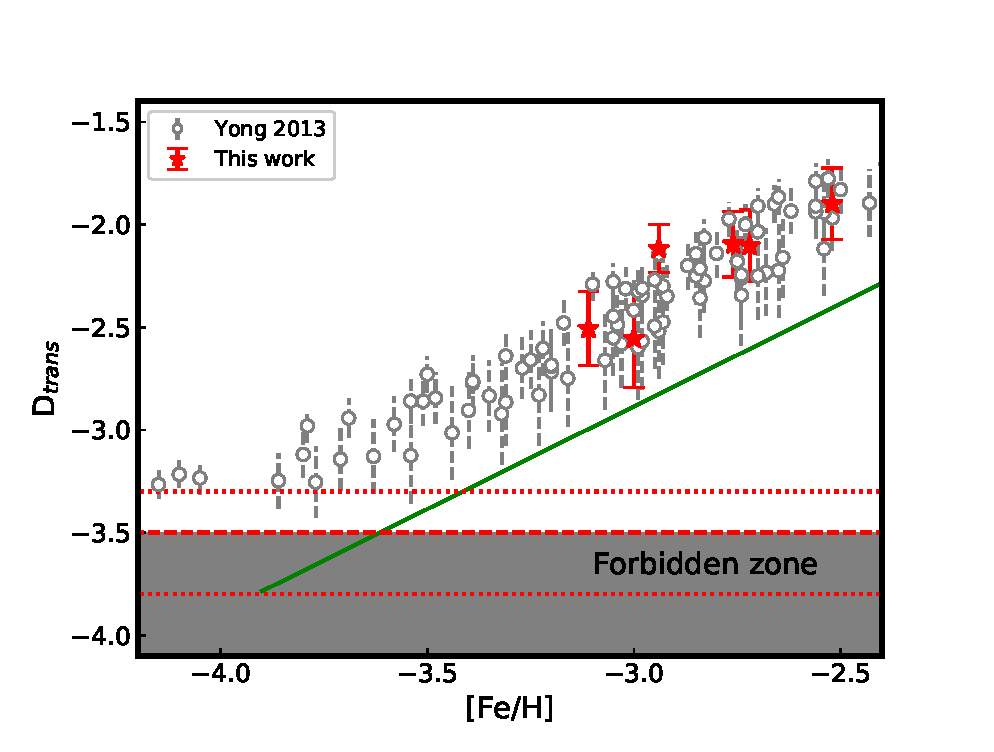
\includegraphics[width=\textwidth, angle=0]{Transition_Discriminant.eps} 
\caption{Dtrans as a function of [Fe/H] for our target stars, compared
with \citet{2013ApJ...762...26Y}. The solid green line denotes the scaled solar
pattern, the red dashed line denotes the limit of Dtrans based on the model
described in Frebel et al. (2007), and the red dotted lines show the uncertainty
of the model. The shaded area is the Forbidden Zone, where there is insufficient
C and O induced cooling for low-mass star formation.}
\label{fig:dtrans}
\end{figure}
  
In addition to the possible nucleosynthesis pathway(s) suggested above, it is
now commonly acknowledged that the formation of Pop II low-mass stars requires
additional coolants compared to the formation of Pop III massive stars
\citep[e.g.,][]{2006ApJ...652....6Y, 2013ASSL..396..103G, 2015ComAC...2....3G}.
At present, a widely acceptable scenario tries to explain the transition from
Pop III to Pop II stars by the notion of the fine-structure cooling of the
\ion{C}{2} and \ion{O}{1} lines \citep[e.g.,][]{2003Natur.425..812B,
2006ApJ...643...26S}. Therefore, C- and O-poor stars can place crucial
constraints on the conditions under which metallicity of the ISM the Pop II
stars may have been formed. 

\citet{2007MNRAS.380L..40F} suggested a criterion for the transition to Pop II
(``transition discriminant" $-$ D$_{trans} = -3.5$) , which combines logarithmic
abundance ratios of [C/H]  and [O/H]. Figure \ref{fig:dtrans}
shows the calculated D$_{trans}$ for our sample stars and carbon-normal stars
adopted from \citet{2013ApJ...762...26Y}. The green solid line denotes the solar
D$_{trans}$ values adopted from \citet{2009ARAA..47..481A}, the red dashed and
the red dotted lines denote the limit of D$_{trans}$ and its associated
uncertainty, respectively, and the gray shaded area represents the Forbidden
Zone. Even though the empirical formula of the D$_{trans}$ requires both
abundances ([C/H] and [O/H]), it is possible to calculate
D$_{trans}$ where only  one of these abundance ratios is known. Here we assume
that [O/Fe] $= 0.88 \pm 0.28$, following the linear relation between the
[C/O] and [C/Fe] suggested by \citet{2004A&A...416.1117C}. We can
notice that our sample stars are located above the solar D$_{trans}$ values and
the Forbidden Zone, suggesting that they may have likely formed from a gas cloud
exhibiting fine-structure cooling process.


\begin{figure}[!ht]
\centering
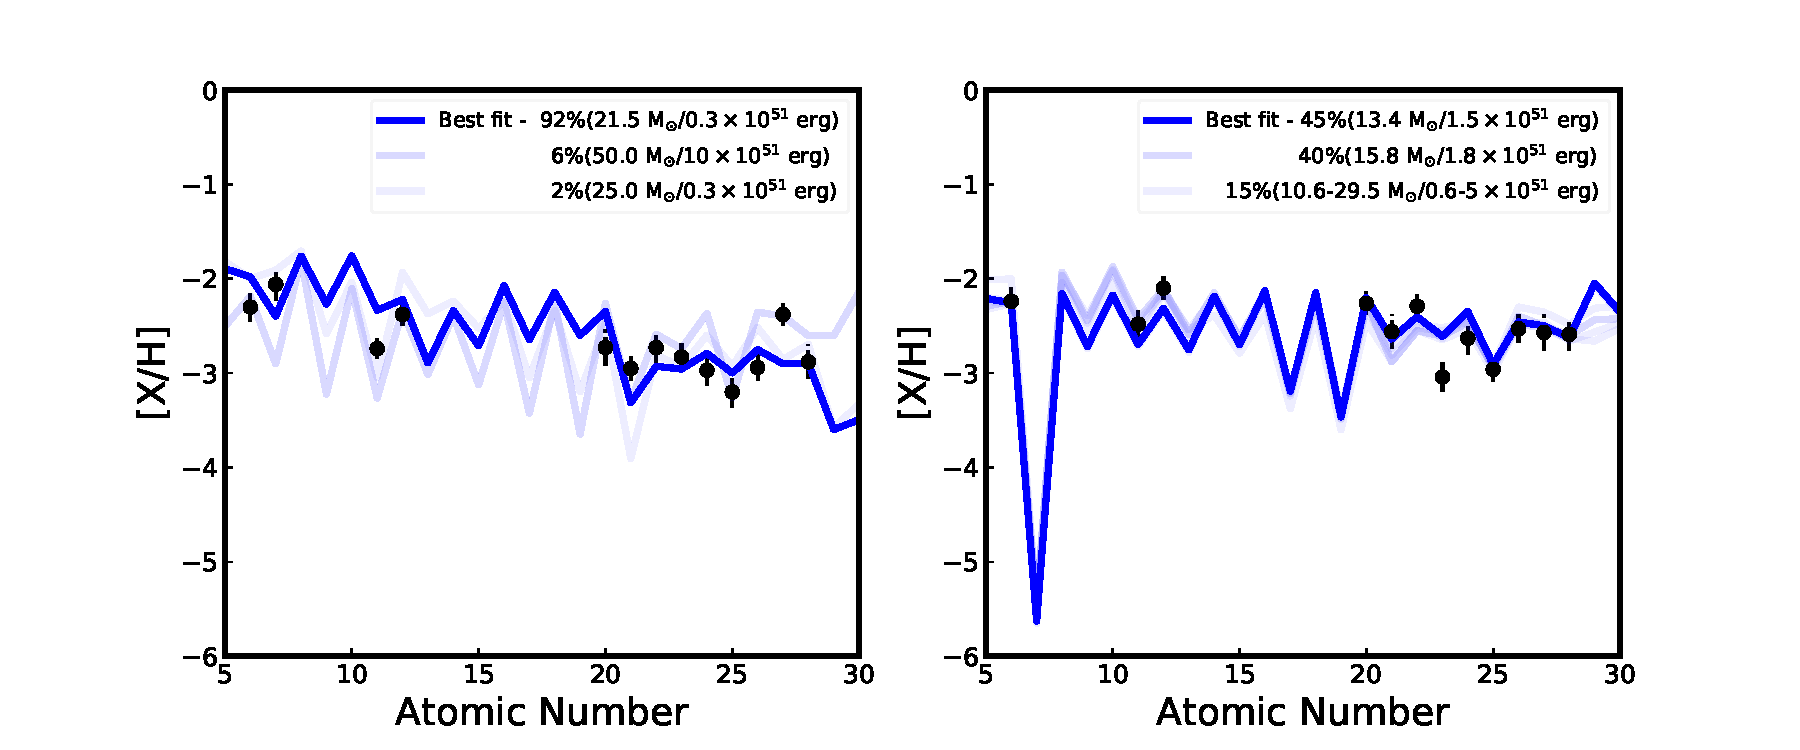
\includegraphics[width=\textwidth, angle=0]{Starfit.pdf} 
\caption{The determined [X/H] abundance ratios of J1630+0953 (left panel)
and J2216+0246 (right panel) as a function of atomic number, overlaid with
simulated abundance patterns by several best fit models, transparent by their
fractional appearance. The best fits and their properties are discussed in the
text.}
\label{fig:starfit}
\end{figure}

\subsection{J1630+0953 and J2216+0246 Possible Progenitors}

Under the assumption that J1630+0953 and J2216+0246 are CEMP-no stars, we
decided to gain insights into their putative progenitors, by comparing their
abundance patterns with theoretical predictions from
\citet[][]{2010ApJ...724..341H}.  For the convenience of the reader, it is worth
mentioning that this grid does not consider rotation and has a $\chi^{2}$
matching algorithm over 16,800 models.  The parameter space includes progenitor
masses (10-100 M$_{\odot}$), explosion energies ($0.3$-$10 \times 10^{51}$ erg),
and mixing factor ($f_{mix}$) ranging from no mixing to nearly complete mixing
\citep[see][for more information]{2010ApJ...724..341H}. 

We sampled $10^{4}$ sets of the determined chemical abundances of J1630+0953 and
J2216+0246, assuming a normal distribution. To facilitate this exercise, we use the
determined log\,$\epsilon$(X) of J1630+0953 and J2216+0246 as the central values
and dispersions given by the associated uncertainties. This allowed us to generate $10^{4}$  abundance patterns
for each star. We use the publicly available \texttt{STARFIT} code
\citep{2010ApJ...724..341H} to find the progenitor mass and explosion energy for
the $10^{4}$ abundance patterns. Figure \ref{fig:starfit}
shows the determined abundances of J1630+0953 and J2216+0246 (black filled
circles), with error bars representing their associated uncertainties,
overlaid with abundance patterns generated by several best fit models.
Figure  \ref{fig:Starfit_histo} shows posterior distributions for the mean
squared residuals of the $10^{4}$ fittings, for both stars. Legends show the
median value and the median absolute deviation (MAD). The MAD can be used as a
robust estimator on how the data spreads out. In other words, the larger the
MAD, the greater the variability in $\chi^{2}$.


\begin{figure}[!ht]
\centering
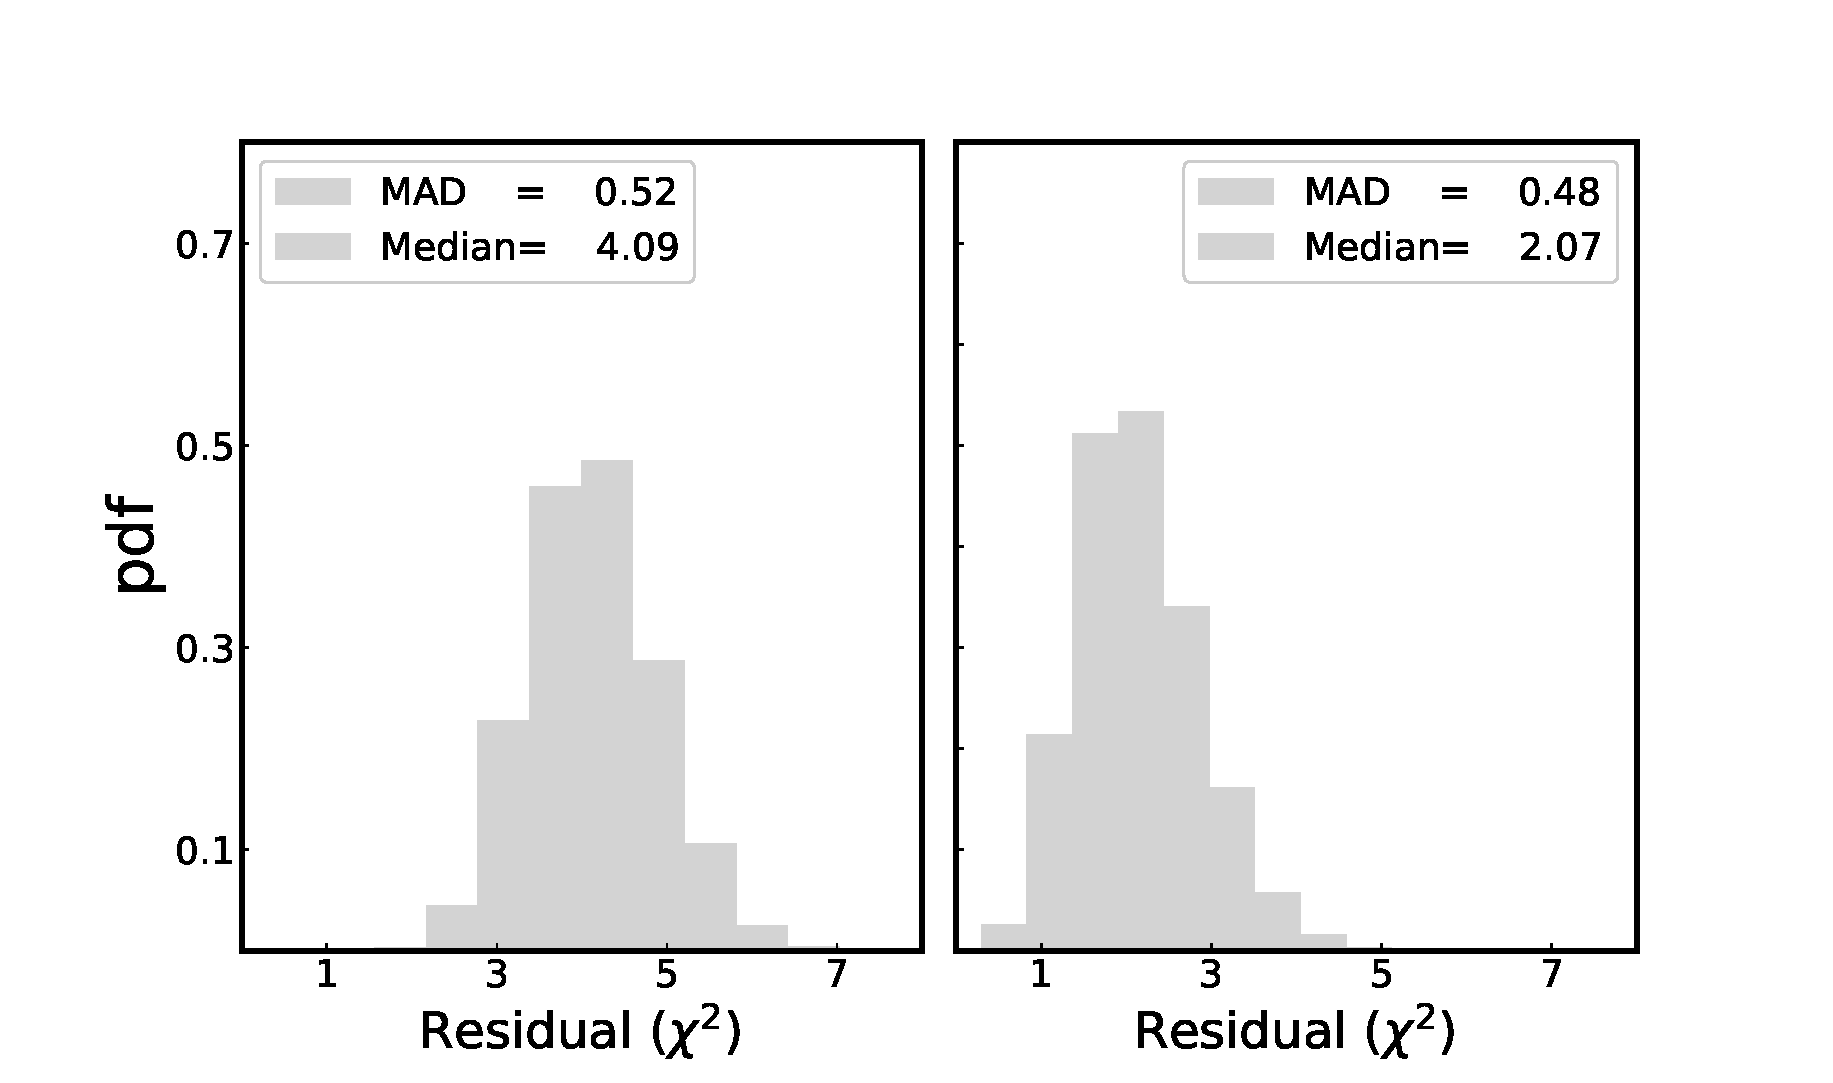
\includegraphics[width=\textwidth, angle=0]{Starfit_histo.eps} 
\caption{Posterior Distributions for $\chi^{2}$, of the 10,000 simulations, for
J1630+0953 (left panel) and J2216+0246 (right panel). The median and median
absolute deviation (MAD) are shown in legends.}
\label{fig:Starfit_histo}
\end{figure}

For J1630+0953, an SN model with mass 21.5 M$_{\odot}$ and explosion energy $0.3
\times 10^{51}$ erg was the most frequent model (92 $\%$) to fit the generated
abundance patterns. Another model with mass 50.0 M$_{\odot}$ and explosion
energy $10.0  \times 10^{51}$ erg fit 6 $\%$ of the generated abundance
patterns, while the remaining of the $10^{4}$ generated abundance patterns (249)
had best fit models with mass 25.0 M$_{\odot}$ and explosion energy $0.3 \times
10^{51}$ erg. 

For J2216+0246, a larger number of SN models were able to fit our $10^{4}$
generated abundance patterns. About 45 $\%$ (4532) of the generated abundance
patterns had best fit with an SN model with mass of 13.4 M$_{\odot}$ and
explosion energy of $1.5 \times 10^{51}$ erg. Another SN model with mass 15.8
M$_{\odot}$ and explosion energy $1.8 \times 10^{51}$ erg was the best fit of 40
$\%$ (3976) of the generated abundance patterns; while 21 different SN models
correspond to the best fit for the rest of the $10^{4}$ generated abundance
patterns (1492). In total, 23 different SN models were the best fits for the
$10^{4}$ generated abundance patterns of J2216+0246, in the mass range 10.6-29.5
M$_{\odot}$ and explosion energies $0.6$-$5 \times 10^{51}$ erg. The abundance
patterns simulated by these 23 models are shown in the right panel of Figure
\ref{fig:starfit}, and color-coded by their fractional appearance.

Regarding the most frequent SN model in the exercise of J1630+0953, it can be
seen through either visual checking or $\chi^{2}$, that the carbon (Z=6) and
nitrogen (Z=7) abundances are well reproduced (within$\sim 2~\sigma$). Sodium
(Z=11) is overproduced, while magnesium (Z=12) is well reproduced (within$\sim
1~\sigma$). Elements from calcium to iron (Z=20-26) are also well reproduced
(within $\sim 2~\sigma$). The cobalt (Z=27) abundance is underproduced, which is
not unusual for theoretical models, where an SN model with higher mass,
explosion energy, and mixing factor may result better Co fitting, although this
could worsen other elements fittings \citep[see][and references
therein]{2014ApJ...785...98T}, while the Nickel (Z=28) is well reproduced. The
predicted yields in  $\sim~85 \%$ of the SN models reproduced the observed
abundances for J2216+0246  within$\sim 2~\sigma$. 

In general, J1630+0953 has possible progenitor with 21-25 M$_{\odot}$ stellar
mass and explosion energy $0.3 \times 10^{51}$ erg, while the mass and
explosion energy of the possible progenitors of J2216+0246 are somewhat lower
(10.6-29.5 M$_{\odot}$, $0.6$-$5 \times 10^{51}$ erg). Recently,
\citet{2018ApJ...857...46I} compared the abundance patterns of 219 EMP stars
with supernova yields of metal-free stars to find that the best fitting
progenitor SNe of most EMP stars are PopIII stars in the range 15-25
M$_{\odot}$. The analysis presented in this paper supports this
hypothesis and suggests that the peak around 20 M$_{\odot}$ may reflect the Pop
III initial mass function and more massive SN might be more energetic that their
ejecta escape from the halo and would never been incorporated into the next
generation of stars.

\subsection{Kinematics and Dynamics} \label{sec:kinematics}

The full space motion of our sample stars can be derived by combining positions
($\alpha$, $\delta$), proper motions ($\mu_{\alpha}\cos\delta$, $\mu_{\delta}$),
available in Gaia DR2 \citep{2018A&A...616A...1G}, the line-of-sight velocities
($V_r$), derived from our high-resolution spectra, and a Galactic potential model. Errors are provided in Gaia
DR2, thus the inversion of the parallax ($\varpi$) to calculate the stellar
distance is not appropriate \citep[see][for a recent
discussion]{2018A&A...616A...9L}.  Therefore, we adopted distances from
\citet[][]{2018AJ....156...58B}, who inferred distances to all stars, with
published parallaxes, in Gaia DR2 using a weak distance prior. Gaia DR2 ID
source, positions, proper motions, distances, and the associated uncertainties
for these quantities. 


\begin{figure}[!ht]
\centering
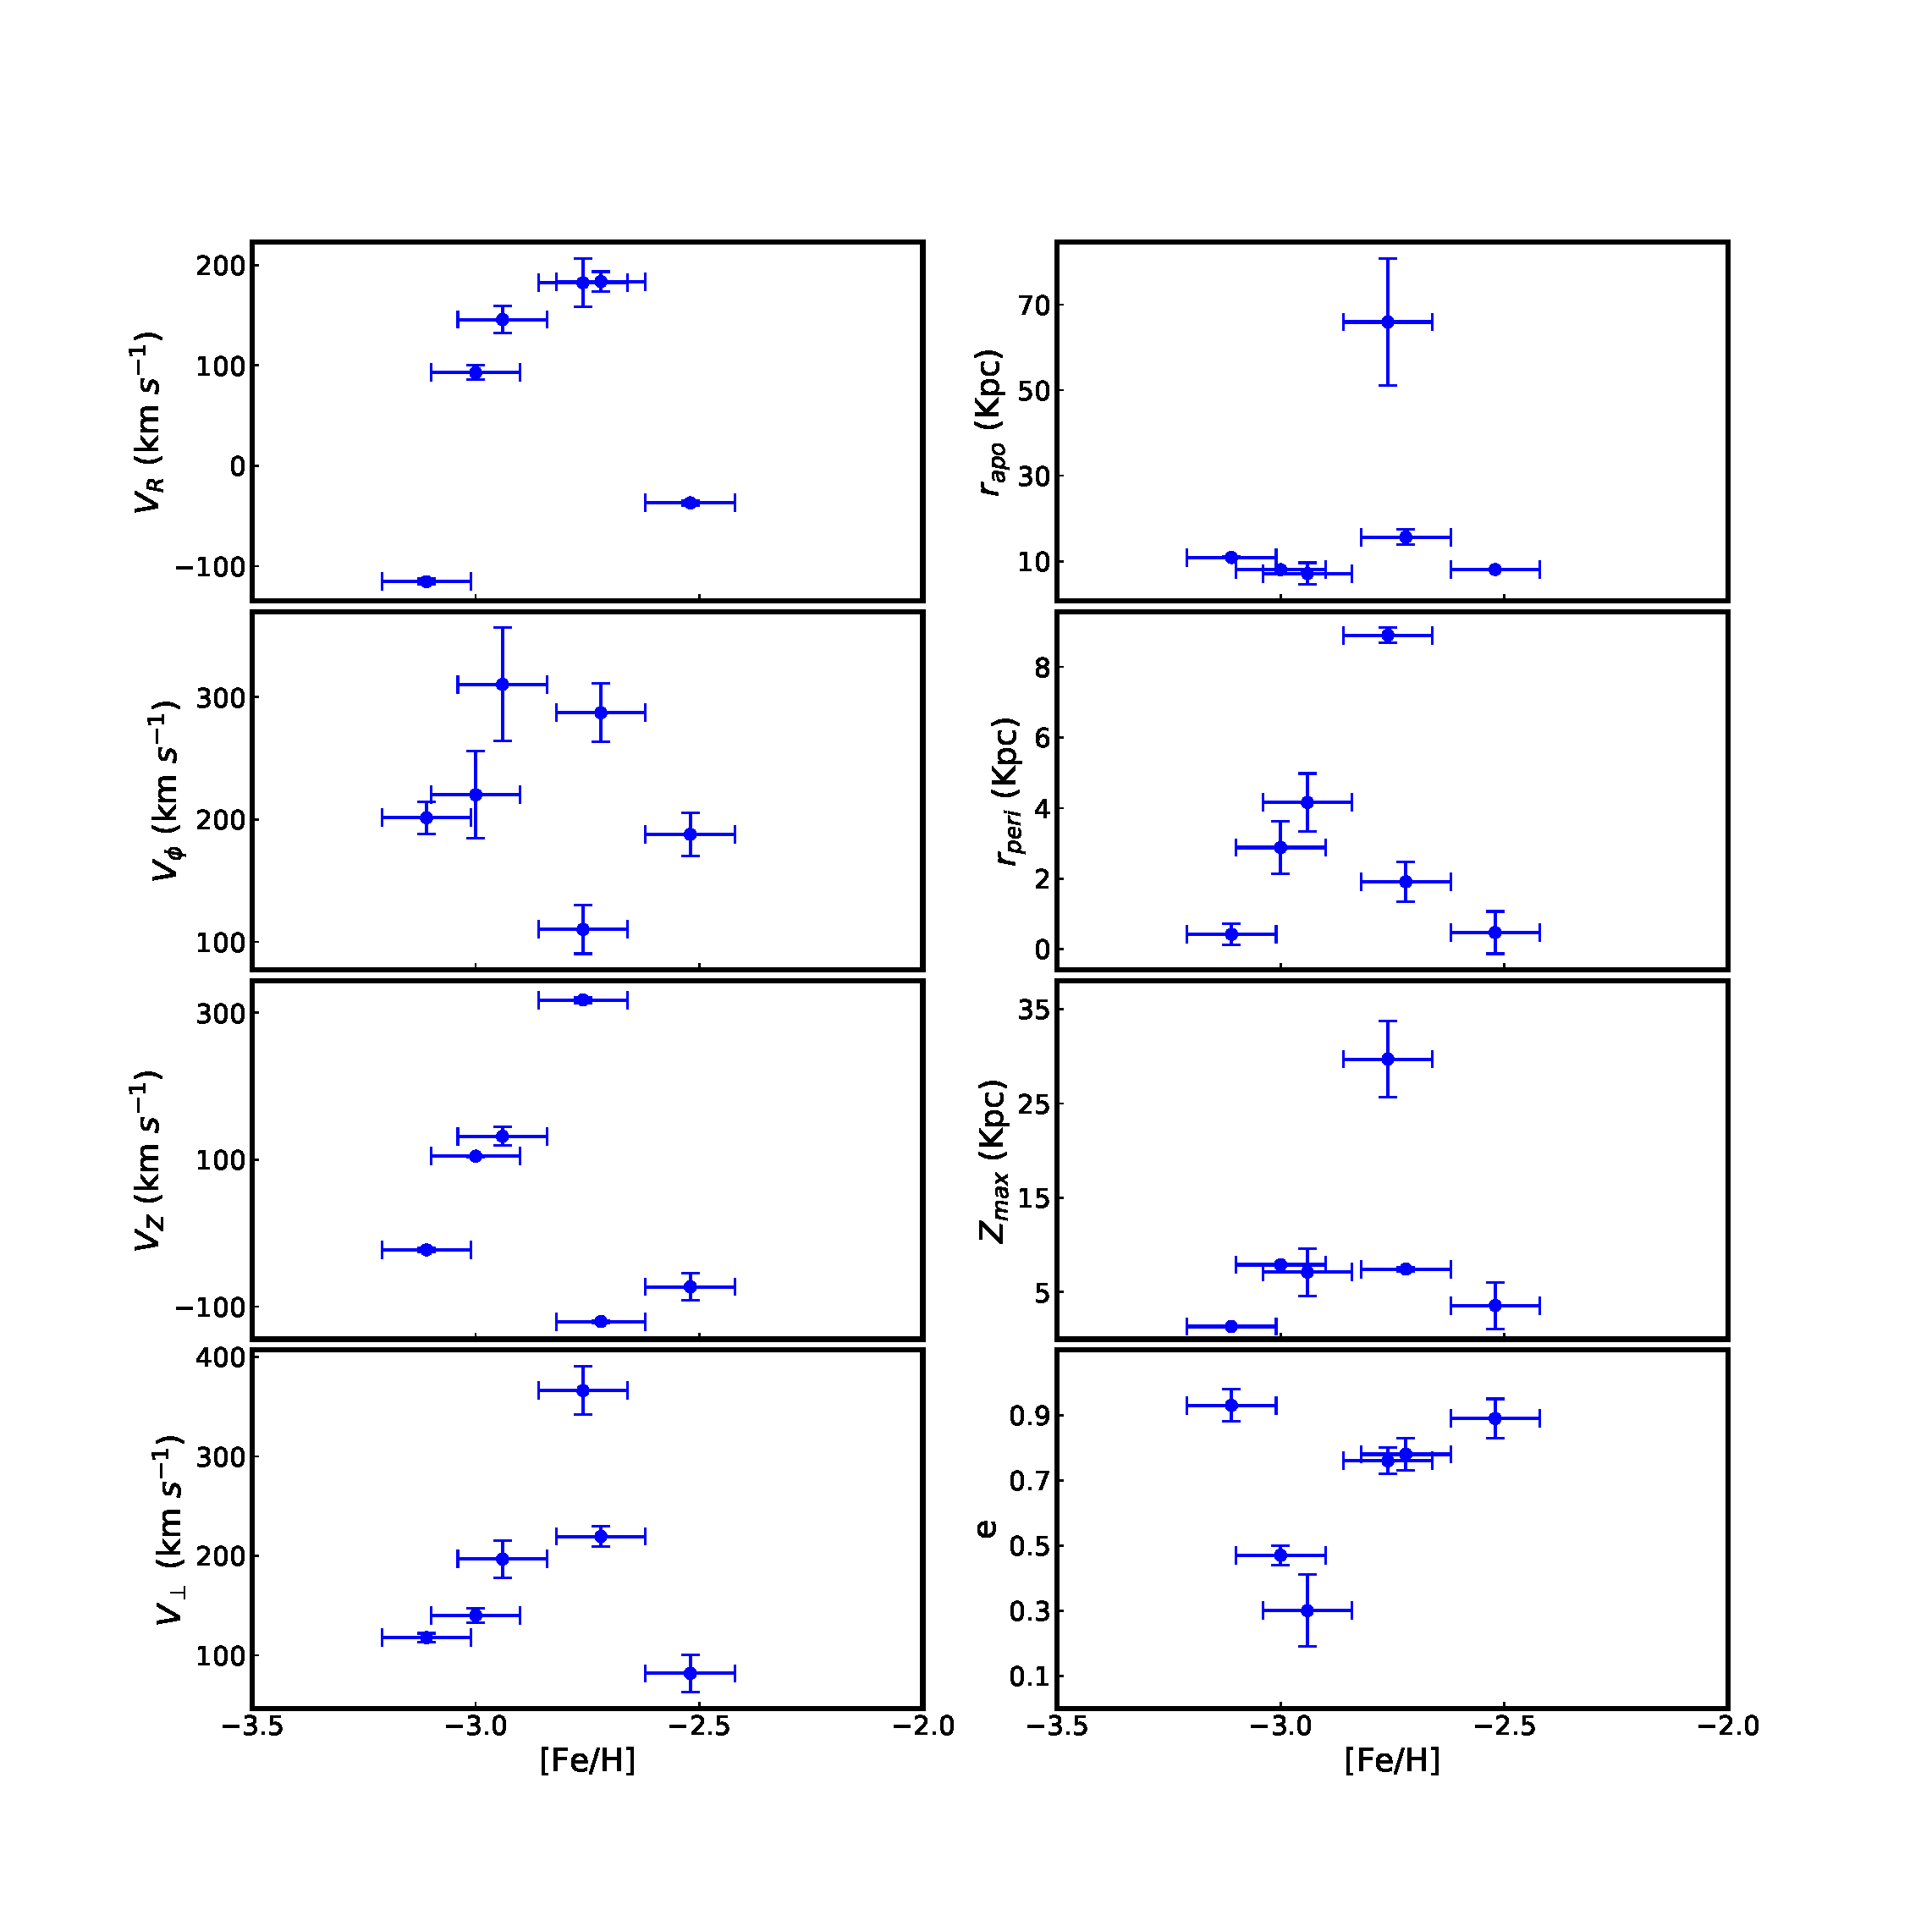
\includegraphics[width=\textwidth, angle=0]{Kinematics.eps} 
\caption{The left panel shows the Galactic velocities and the right panel shows
the orbital parameters for our sample stars as functions of [Fe/H]. The
y-axis error bars denote the 16$^{\rm th}$ and 84$^{\rm th}$ percentiles, while
the x-axis error bars represent a typical [Fe/H] uncertainty (0.10
$\sim$dex).}
\label{fig:Kinematics}
\end{figure}

We sampled $10^{4}$ sets of the observed astrometric quantities (RA, DEC,
$\varpi$, RV, $\mu_{\alpha}\cos\delta$, $\mu_{\delta}$) from the measurement
errors of each quantity for each star in our sample. We assume that the Sun has an offset above the
Galactic midplane of $z_{\odot}= 25$ pc \citep{2008ApJ...673..864J}, $R_{\odot}
=$~8.2~kpc \citep{2016ARA&A..54..529B} as the distance from the Galactic center,
circular velocity $v_0 =$~232.8~\mbox{km~s$^{\rm -1}$} at the Solar position
\citep{ 2017MNRAS.465...76M}, and solar peculiar motion $(U_\odot, V_\odot,
W_\odot) =$ (11.1, 12.24, 7.25)~\mbox{km~s$^{\rm -1}$}
\citep{2016ARA&A..54..529B}.  We calculate the Galactocentric Cartesian
($X_{GC}, Y_{GC}, Z_{GC}$) coordinates as follows:

\begin{eqnarray*} \label{eq:xyz}
X_{GC}  & = & R_{\odot} - d \cos (b) \cos (\ell) \\
Y_{GC}  & = &- d \cos (b) \sin (\ell)  \\
Z_{GC}  & = & d \sin (b) + z_{\odot}\\
\end{eqnarray*}

We calculated and corrected the Galactic space-velocity components $(U, V, W)$
using the Astropy Galactocentric frame package \citep{2013A&A...558A..33A,
2018AJ....156..123A}: U (positive toward the Galactic center), V (positive in
the direction of Galactic rotation) and W (positive toward the North Galactic
Pole).  Moreover, we define the angle $\phi = \tan^{-1}(Y_{GC}/X_{GC})$ and then
calculate the cylindrical velocities components for our sample as follows:

 \begin{eqnarray*} \label{eq:xyz}
V_{R}    & = & U \cos (\phi) + V \sin (\phi)\\
V_{\phi} & = & U \sin (\phi) - V \cos (\phi) \\
V_{z}     & = & W \\
\end{eqnarray*}

We adopted the \texttt{MWPotential2014} as a Galactic potential model
\citep[see][for more information]{2015ApJS..216...29B} to integrate the
corresponding stellar orbits, apocentric ($\rapo$) and pericentric ($\rperi$)
radii, the maximum offset from the Galactic midplane ($\zmax$), and
eccentricity, defined as $e = (\rapo - \rperi) / (\rapo + \rperi)$. In addition,
we derived the total orbital energy, defined as $E = (1/2) \vector{v}^2 +
\Phi(\vector{x})$ and the angular momentum in the vertical direction, defined as
$L_z = R \times V_{\phi}$, where $R$ denotes the distance from the Galactic
center projected onto the disk plane.


Figure \ref{fig:Kinematics} shows the behavior of the calculated velocities and
orbital properties, for our sample stars, as a function of [Fe/H]. Error
bars denote typical [Fe/H] uncertainty (x-axis) and the 16th and 84th
percentiles (y-axis). It is possible to see that 66 $\%$ of our sample is moving
away (V$_{R} >0$) from the Galactic center, 100$\%$ on prograde (V$_{\phi} >0$)
orbits, and 50 $\%$ moving north (V$_{Z} >0$), as they pass through the Galactic
disk. The right panel shows that only J1108+2530 and J1256+3440 have $\rapo >
15.0$ kpc and $e > 0.7$ and the majority of our sample stars pass the Galactic
center at $\rperi=4.16$. Also, 66$\%$ of our sample stars travel at least 7 kpc
above or below the Galactic plane. 

An additional tool that can be used for this analysis is the Lindblad diagram.
By plotting the total orbital energy vs. angular momentum in the vertical
direction, one can assess the accretion origin of the sample stars. \citet{2014ApJ...788..180C} explored
kinematics, integrals of motion, and orbital properties of 323 VMP stars, to
establish a method to assign membership to the inner- and outer-halo
populations. In this context, stars with total energy $> -0.9$ km$^{2}$ s$^{-2}$
and $\rapo~>15$ kpc can be considered as outer-halo stars. Otherwise, stars can
be considered as members of the inner-halo population.
  

\begin{figure}[!ht]
\centering
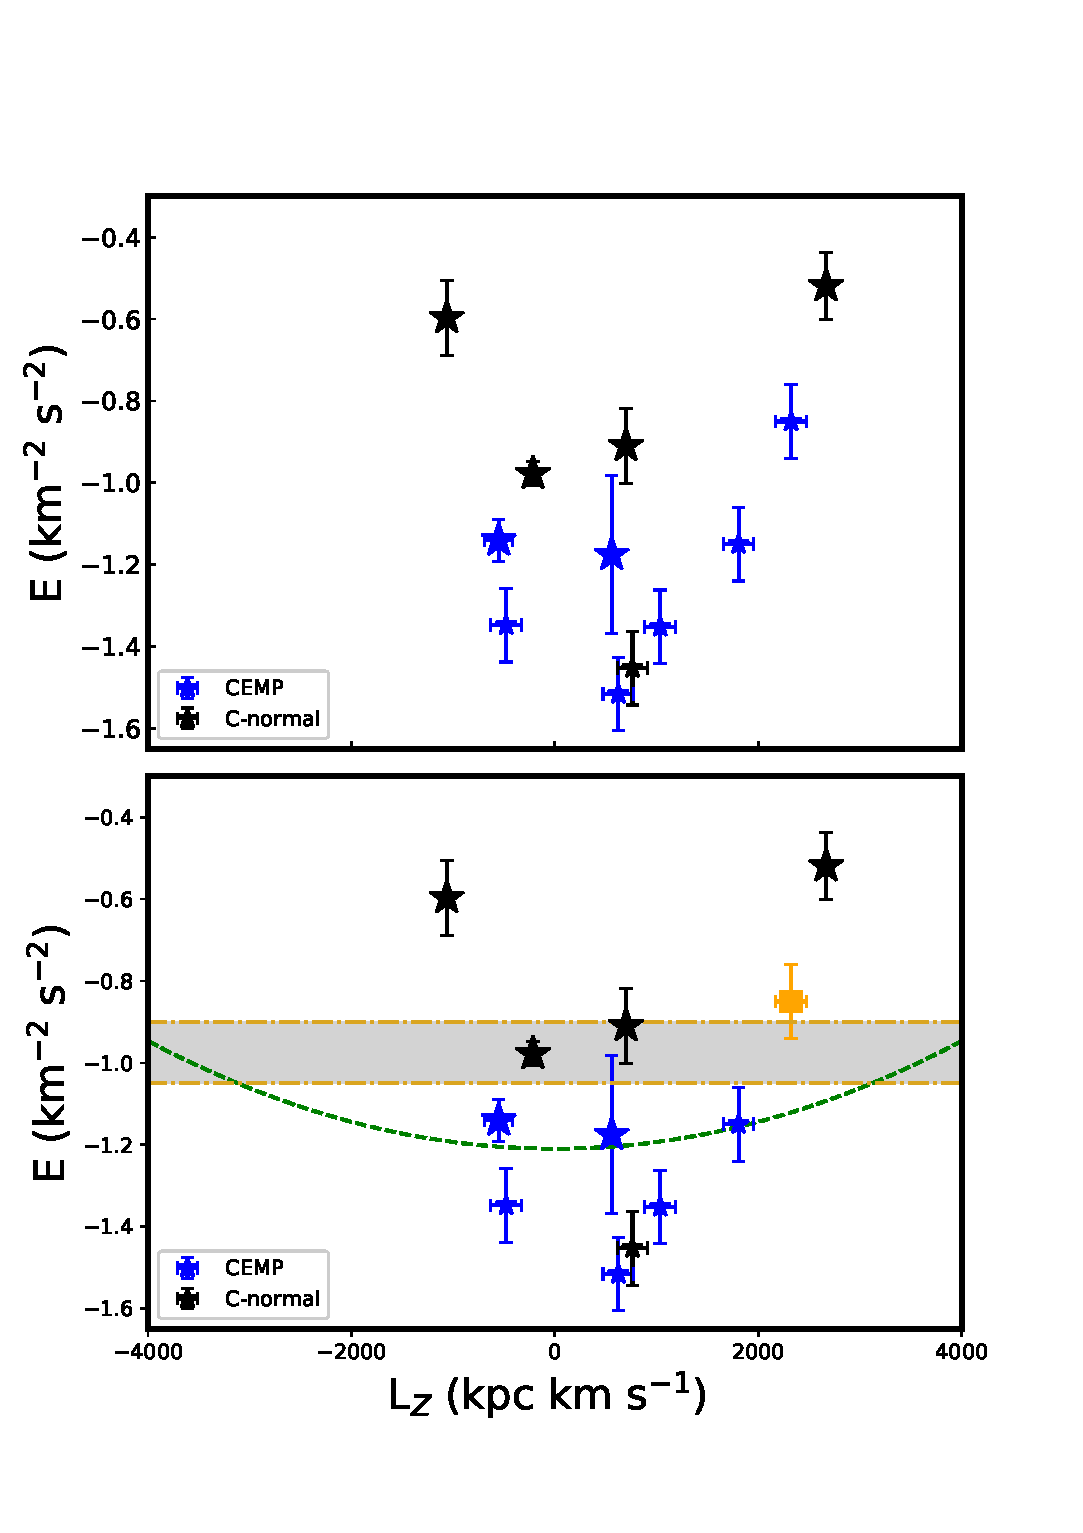
\includegraphics[width=\textwidth, angle=0]{Energy_L_Z.eps} 
\caption{Lindblad diagram for program stars and data taken from Paper I. Top
panel shows the distribution of this sample based on [C/Fe] abundance
ratios, carbon normal (black stars) and CEMP stars (red stars). Bottom panel
shows the distribution of this sample based on \citet{2014ApJ...788..180C}
criterion. CEMP-no stars are shown as blue filled star, CEMP-r/s as orange
filled square, and C-normal stars as black filled star. The green dashed curve
represents the locus of the points that possess constant apo-Galactic radius,
rapo = 15 kpc. The light-gray shaded area encloses the transition zone
energies.}
\label{fig:Lindblad}
\end{figure}

Figure \ref{fig:Lindblad} shows the Lindblad diagram (top panel) and the
\citet{2014ApJ...788..180C} criterion (bottom panel) for the sample stars,
compared to stars taken from Paper I. CEMP-no stars are shown as blue filled
stars, CEMP-r/s star as orange filled square, and C-normal stars as black filled
stars. The green dashed curve represents the locus of the points that possess
constant apo-Galactic radius, $\rapo = 15$ kpc. The light-gray shaded area
encloses the transition zone energies. It is possible to see that J1630+0953
and J2216+0246, within the error bars, are likely to have inner-halo kinematics. 

Many numerical cosmological simulations suggest that the main origin of the
Milky Way inner and outer-halo stars are massive and low-mass subgalactic fragments,
respectively \citep{2009ApJ...702.1058Z,2011MNRAS.416.2802F,2012MNRAS.420.2245M,
2012AAS...21922206B,  2013MNRAS.432.3391T, 2014MNRAS.439.3128T}. In general, We
can understand the origin of our stars by examining a combination of their
orbital parameters and integrals of motion. The derived orbital parameters and
the calculated total energy of J1630+0953 and J2216+0246 suggest that they
probably belong to the inner-halo population. However, their metallicity
and C-enhancement indicate that they may have formed not in situ but in small
mass subgalactic fragments that were accreted very early on and contributed to
the old central regions of the halo system
\citep[e.g.,][]{2018MNRAS.473.1656T}.
